%%%%%%%%%%%%%%%%%%%%%%%%%%%%%%%%%%%%%%%%%
% Beamer Presentation
% LaTeX Template
% Version 1.0 (10/11/12)
%
% This template has been downloaded from:
% http://www.LaTeXTemplates.com
%
% License:
% CC BY-NC-SA 3.0 (http://creativecommons.org/licenses/by-nc-sa/3.0/)
%
%%%%%%%%%%%%%%%%%%%%%%%%%%%%%%%%%%%%%%%%%

%----------------------------------------------------------------------------------------
%	PACKAGES AND THEMES
%----------------------------------------------------------------------------------------

\documentclass{beamer}
%--------This section sets up the document class and packages.
\usepackage[includeheadfoot, margin=20mm, headheight=20mm]{geometry} 
\usepackage{fancyhdr}
\usepackage{mwe}
\usepackage{amsmath}
\usepackage{amsthm}
\usepackage[utf8]{inputenc}
\usepackage{amssymb}
%\usepackage{xcolor,graphicx}
\usepackage{hyperref}
\usepackage{centernot}
\usepackage{tikz}  % Uncomment this line iff you are using the tikz package to add drawings
\usepackage{tkz-euclide}
\usepackage{pgf}
\usepackage{pgfplots}
\pgfplotsset{compat=newest}
\pgfplotsset{plot coordinates/math parser=false}
\usepackage[toc,page]{appendix}
\usepackage{hyperref}
\usepackage{pdfpages}
\usepackage{xargs}                      % Use more than one optional parameter in a new commands
%\usepackage[pdftex,dvipsnames]{xcolor}  % Coloured text etc.
% 
\usepackage[colorinlistoftodos,prependcaption]{todonotes}
\newcommandx{\unsure}[2][1=]{\todo[linecolor=red,backgroundcolor=red!25, size=\small,bordercolor=red,#1]{#2}}
\usepackage{url}
\usepackage[ruled,vlined]{algorithm2e}
\SetKwComment{Comment}{$\triangleright$\ }{}
\usepackage{listings}

\allowdisplaybreaks
\pgfplotsset{soldot/.style={color=blue,only marks,mark=*}} \pgfplotsset{holdot/.style={color=blue,fill=white,only marks,mark=*}}

\usepackage{tocloft}
\renewcommand{\cftsecleader}{\cftdotfill{\cftdotsep}}
\renewcommand\labelenumi{(\roman{enumi})}

%--- This section makes possible customized theorem numbering.
\newtheorem{innercustomgeneric}{\customgenericname}
\providecommand{\customgenericname}{}
\newcommand{\newcustomtheorem}[2]{%
  \newenvironment{#1}[1]
  {%
   \renewcommand\customgenericname{#2}%
   \renewcommand\theinnercustomgeneric{##1}%
   \innercustomgeneric
  }
  {\endinnercustomgeneric}
}
\newcustomtheorem{cthm}{Theorem}
\newcustomtheorem{caxm}{Axiom}
\newcustomtheorem{clem}{Lemma}
\newcustomtheorem{ccor}{Corollary}
\newcustomtheorem{cprop}{Proposition}
\newcustomtheorem{cdefn}{Definition}
\newcustomtheorem{ceg}{Example}
\newcustomtheorem{crmk}{Remark}
\newcustomtheorem{ccus}{}
\newcustomtheorem{cprob}{Problem}

%---The following code sets up the way theorems are typeset and labeled.
\newtheorem{thm}{Theorem}
\newtheorem{lem}[thm]{Lemma}
\newtheorem{cor}[thm]{Corollary}
\newtheorem{prop}[thm]{Proposition}
\theoremstyle{definition}
\newtheorem{defn}[thm]{Definition}
\newtheorem{axm}[thm]{Axiom}
\newtheorem{eg}[thm]{Example}
\theoremstyle{remark}
\newtheorem{rmk}[thm]{Remark}
\newtheorem{sol}{Solution}

% \numberwithin{equation}{subsection}
% \numberwithin{thm}{section}

% \newtheorem*{thm}{Theorem}
% \newtheorem*{lem}{Lemma}
% \newtheorem*{cor}{Corollary}
% \newtheorem*{prop}{Proposition}
% \theoremstyle{definition}
% \newtheorem*{defn}{Definition}
% \newtheorem*{axm}{Axiom}
% \newtheorem*{eg}{Example}
% \theoremstyle{remark}
% \newtheorem*{rmk}{Remark}
% \newtheorem*{sol}{Solution}


%---The following code defines a few extra commands that will be useful in some exercises.
\newcommand{\abs}[1]{\lvert#1\rvert}     % Absolute value symbol
\newcommand{\Abs}[1]{\Bigg\lvert#1\Bigg\rvert}     % Absolute value symbol (big)
\newcommand{\Z}{\mathbb Z}              % The set of integers
\newcommand{\Q}{\mathbb Q}              % The set of rationals
\newcommand{\R}{\mathbb R}              % The set of reals
\newcommand{\N}{\mathbb N}              % The set of natural numbers
\newcommand{\C}{\mathbb C}              % The set of complex numbers
\newcommand{\F}{\mathbb F}  

\newcommand{\ZZ}{\mathcal{Z}}
\newcommand{\OO}{\mathcal{O}}
\newcommand{\CC}{\mathcal{C}}
\newcommand{\UU}{\mathcal{U}}
\newcommand{\power}{\mathcal{P}}         % The power set of a set
\newcommand{\bfun}{\mathcal{F}}          % The finite subsets
\newcommand{\Id}{\mathrm{Id}}            % The identity function
\newcommand{\nil}{\emptyset}             % Empty set
\newcommand{\inflim}[1]{\lim_{#1\to\infty}} % Limit to infinity
\newcommand{\ninflim}[1]{\lim_{#1\to\infty}}% Limit to negative infinity
\providecommand{\BVec}[1]{\mathbf{#1}}   % Bold font for vectors
\DeclareMathOperator{\gon}{gon}          % A polygon
\DeclareMathOperator{\Fun}{Fun}          % The set of all functions from one set to another
\DeclareMathOperator{\Perm}{Perm}        % The set of all permutations on a set
\DeclareMathOperator{\Int}{int} %interior of a set
\DeclareMathOperator{\cl}{cl} %closure of a set
\DeclareMathOperator{\diam}{diam}
\DeclareMathOperator{\sinc}{sinc}
\DeclareMathOperator{\rank}{rank}
\DeclareMathOperator{\Span}{span}
\DeclareMathOperator{\len}{length}
%\newcommand{\Re}{\mathrm{Re}} %real part

\providecommand{\LIN}[1]{{\color{blue}#1}} %Linda's notes

% Dave's macros
\definecolor{colorDAS}{RGB}{255,127,0}
\providecommand{\DAS}[1]{{\color{colorDAS}#1}}     % Dave's comments

\usetheme{Madrid}
\useoutertheme{miniframes} % Alternatively: miniframes, infolines, split
\useinnertheme{rectangles}

% \definecolor{UBCblue}{rgb}{0.04706, 0.13725, 0.26667} % UBC Blue (primary)
% \definecolor{UBCgrey}{rgb}{0.3686, 0.5255, 0.6235} % UBC Grey (secondary)

% \setbeamercolor{palette primary}{bg=UBCblue,fg=white}
% \setbeamercolor{palette secondary}{bg=UBCblue,fg=white}
% \setbeamercolor{palette tertiary}{bg=UBCblue,fg=white}
% \setbeamercolor{palette quaternary}{bg=UBCblue,fg=white}
% \setbeamercolor{structure}{fg=UBCblue} % itemize, enumerate, etc
% \setbeamercolor{section in toc}{fg=UBCblue} % TOC sections

% % Override palette coloring with secondary
% \setbeamercolor{}{bg=UBCgrey,fg=white}

\mode<presentation> {
    \usefonttheme{professionalfonts}
% The Beamer class comes with a number of default slide themes
% which change the colors and layouts of slides. Below this is a list
% of all the themes, uncomment each in turn to see what they look like.

%\usetheme{default}
%\usetheme{AnnArbor}
%\usetheme{Antibes}
%\usetheme{Bergen}
%\usetheme{Berkeley} % side toc
%\usetheme{Berlin}
%\usetheme{Boadilla}
%\usetheme{CambridgeUS}
%\usetheme{Copenhagen}
%\usetheme{Darmstadt}
%\usetheme{Dresden}
%\usetheme{Frankfurt}
%\usetheme{Goettingen} % side toc on the right
%\usetheme{Hannover} % side toc
%\usetheme{Ilmenau}
%\usetheme{JuanLesPins}
%\usetheme{Luebeck}
%\usetheme{Madrid}
%\usetheme{Malmoe}
%\usetheme{Marburg} % side toc on the right
%\usetheme{Montpellier}
%\usetheme{PaloAlto} % side toc
%\usetheme{Pittsburgh}
%\usetheme{Rochester}
%\usetheme{Singapore}
%\usetheme{Szeged}
%\usetheme{Warsaw}

% As well as themes, the Beamer class has a number of color themes
% for any slide theme. Uncomment each of these in turn to see how it
% changes the colors of your current slide theme.

%\usecolortheme{albatross}
%\usecolortheme{beaver}
%\usecolortheme{beetle}
%\usecolortheme{crane}
%\usecolortheme{dolphin}
\usecolortheme{dove} % black and white
%\usecolortheme{fly}
%\usecolortheme{lily}
%\usecolortheme{orchid}
%\usecolortheme{rose}
%\usecolortheme{seagull}
%\usecolortheme{seahorse}
%\usecolortheme{whale}
%\usecolortheme{wolverine}

\setbeamertemplate{headline}
%\setbeamertemplate{footline} % To remove the footer line in all slides uncomment this line
%\setbeamertemplate{footline}[page number] % To replace the footer line in all slides with a simple slide count uncomment this line

\setbeamertemplate{navigation symbols}{} % To remove the navigation symbols from the bottom of all slides uncomment this line
}

\setbeamertemplate{title page}[default][colsep=-4bp,rounded=true]
\setbeamertemplate{frametitle}[default][colsep=-4bp,rounded=false,shadow=false]
\setbeamertemplate{blocks}[default]
\setbeamercolor{block title}{bg=gray!20}
%\setbeamercolor{block title}{bg=white}
\setbeamercolor{block body}{bg=white}
\setbeamerfont{block title}{size=\small}
\setbeamerfont{block body}{size=\small}

\setbeamerfont{bibliography item}{size=\footnotesize}
\setbeamerfont{bibliography entry author}{size=\footnotesize}
\setbeamerfont{bibliography entry title}{size=\footnotesize}
\setbeamerfont{bibliography entry location}{size=\footnotesize}
\setbeamerfont{bibliography entry note}{size=\footnotesize}

\let\oldfootnotesize\footnotesize
\renewcommand*{\footnotesize}{\oldfootnotesize\tiny}

\setbeamertemplate{caption}[numbered]
\setbeamertemplate{frametitle continuation}{}

\usepackage{graphicx} % Allows including images
\usepackage{booktabs} % Allows the use of \toprule, \midrule and \bottomrule in tables
%\usepackage{bibentry}
\usepackage[style=verbose, backend=bibtex]{biblatex}
\addbibresource{C:/Bibtex/Capstone}

\usepackage{tcolorbox}

%----------------------------------------------------------------------------------------
%	TITLE PAGE
%----------------------------------------------------------------------------------------

\title[]{Algorithmic Solution of \\High Order Partial Differential Equations\\in Julia\\ via the Fokas Transform Method} % The short title appears at the bottom of every slide, the full title is only on the title page

\author[]{\textcolor{gray}{Linfan Xiao}} % Your name
\institute[] % Your institution as it will appear on the bottom of every slide, may be shorthand to save space
{
Advisor: Prof. Dave Smith\\
Mathematical, Computational, and Statistical Sciences\\
Yale-NUS College \\ % Your institution for the title page
\medskip
%\textit{linfan.xiao@u.yale-nus.edu.sg} % Your email address
}
\date[]{\today} % Date, can be changed to a custom date

\begin{document}
%\bibliographystyle{utphys}
%\nobibliography{C:/Bibtex/Capstone}
%\bibliography{C:/Bibtex/Capstone}

\begin{frame}
\titlepage % Print the title page as the first slide
\end{frame}

\begin{frame}[t]
    \begin{tcolorbox}[colback=white,colframe=gray!40, arc=0pt, outer arc=0pt]
        \begin{center}
            \Large Algorithmic Solution of \\
            High Order Partial Differential Equations\\
            in Julia\\
            via the Fokas Transform Method
        \end{center}
    \end{tcolorbox}
    % \noindent\makebox[\linewidth]{\rule{\paperwidth}{0.4pt}}
\end{frame}

\begin{frame}[t]
    \begin{tcolorbox}[colback=white,colframe=gray!40, arc=0pt, outer arc=0pt]
        \begin{center}
            \Large {\color{lightgray}Algorithmic Solution of \\
            High Order} Partial Differential Equations$^*$\\
            {\color{lightgray}in Julia\\
            via the Fokas Transform Method}
        \end{center}
    \end{tcolorbox}
    \begin{itemize}
        \item[$*$] Equations of the form 
        \[f\left(x_1,\ldots, x_n, u, u_{x_1},\ldots,u_{x_n},u_{x_1 x_1},\ldots,u_{x_1 x_n},\ldots \right) = 0,\]
        which relate an unknown function $u(x_1,\ldots,x_n)$ to its partial derivatives $u_{x_i\cdots x_j} := \frac{\partial}{\partial x_i}\cdots \frac{\partial}{\partial x_j}u$.
    \end{itemize}
\end{frame}

\begin{frame}[t]
    \begin{tcolorbox}[colback=white,colframe=gray!40, arc=0pt, outer arc=0pt]
        \begin{center}
            \Large Algorithmic Solution {\color{lightgray}of \\
            High Order Partial Differential Equations\\
            in Julia}\\
            via the Fokas Transform Method$^*$
        \end{center}
    \end{tcolorbox}
    
    \begin{itemize}
        \item[$*$] A method to solve a certain class of PDE problems algorithmically\footcite{Fokas2008}.
    \end{itemize}
\end{frame}

\begin{frame}[t]
    \begin{tcolorbox}[colback=white,colframe=gray!40, arc=0pt, outer arc=0pt]
        \begin{center}
            \Large{\color{lightgray}Algorithmic Solution of \\
            High Order Partial Differential Equations}\\
            in Julia$^*$\\
            {\color{lightgray}via the Fokas Transform Method}
        \end{center}
    \end{tcolorbox}

    \begin{itemize}
        \item[$*$] A free, open-source, high-performance language for numerical computing\footcite{julia}.
    \end{itemize}
\end{frame}

\begin{frame}
    \frametitle{Table of Contents} % Table of contents slide, comment this block out to remove it
    \tableofcontents % Throughout your presentation, if you choose to use \section{} and \subsection{} commands, these will automatically be printed on this slide as an overview of your presentation
\end{frame}

\section{Motivation}

\begin{frame}
    \frametitle{Motivation}
    \begin{itemize} \setlength\itemsep{1em}
        \item PDEs can model various physical phenomena. E.g.,
        \begin{itemize}
            \item heat equation $u_t = Ku_{xx}$
            \item wave equation $u_{tt} = c^2(u_{xx}+u_{yy})$
            \item (linear) Schr\"{o}dinger equation $ihw_t + \frac{h}{2m}w_{xx}=0$
        \end{itemize}
        \item Problems involving PDEs are usually formulated as initial-boundary value problems (IBVPs), consisting of
        \begin{itemize}
            \item a PDE in temporal and spatial variables defined over a domain,
            \item boundary conditions, and
            \item initial condition.
        \end{itemize}
        % E.g., the one-dimensional heat equation 
        % \[u_t = Ku_{xx},\quad (x,t)\in (0, L)\times (0,\infty)\]
        % with periodic boundary conditions
        % \begin{alignat*}{3}
        %     u(0, t) &= u(L, t),&\quad t&\in (0,\infty)\\
        %     u_x(0, t) &= u_x(L, t),&\quad t&\in (0,\infty)
        % \end{alignat*}
        % and initial condition 
        % \[u(x,0) = f(x), \quad x\in (0, L).\]
    \end{itemize}
\end{frame}

\begin{frame}
    \frametitle{Motivation}
    \begin{itemize}
        \item Some IBVPs can be solved using classical transform pairs, e.g., the Fourier transform. 
    \end{itemize}
    \begin{figure}[htpb!]
        \centering
        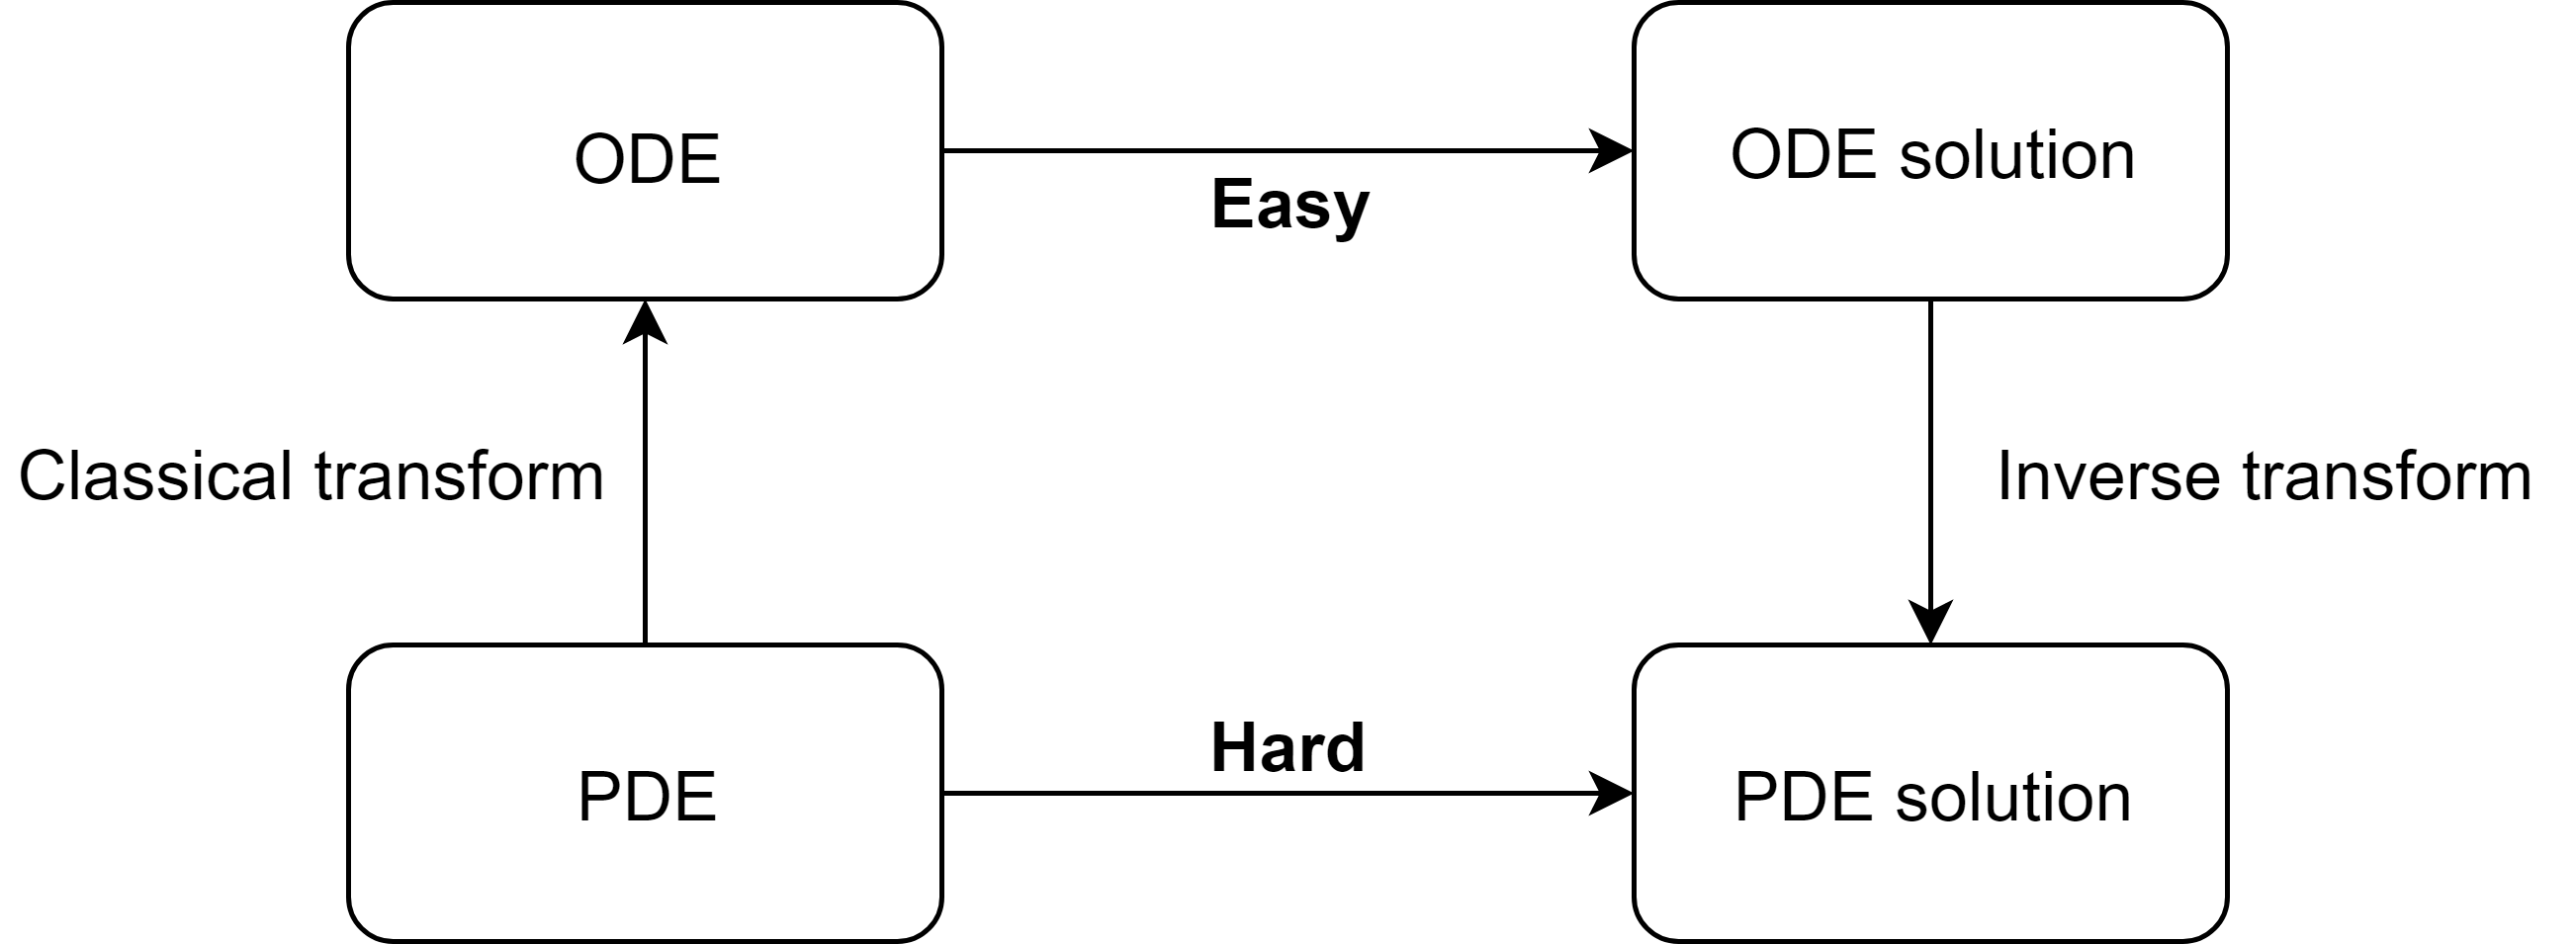
\includegraphics[width=1\textwidth]{classical_transform.png}
        %\caption{Solving IBVPs using classical transform pairs, e.g., the Fourier transform.}
        \label{fig:classical_transform}
    \end{figure}
\end{frame}

\begin{frame}
    \frametitle{Motivation}
    \begin{itemize}
        \item For more complicated IBVPs, no such classical transform pairs exist. 
        \begin{itemize}
            \item Resort to ad-hoc methods that are specific to the given IBVP.
        \end{itemize}
    \end{itemize}
    \begin{figure}[htpb!]
        \centering
        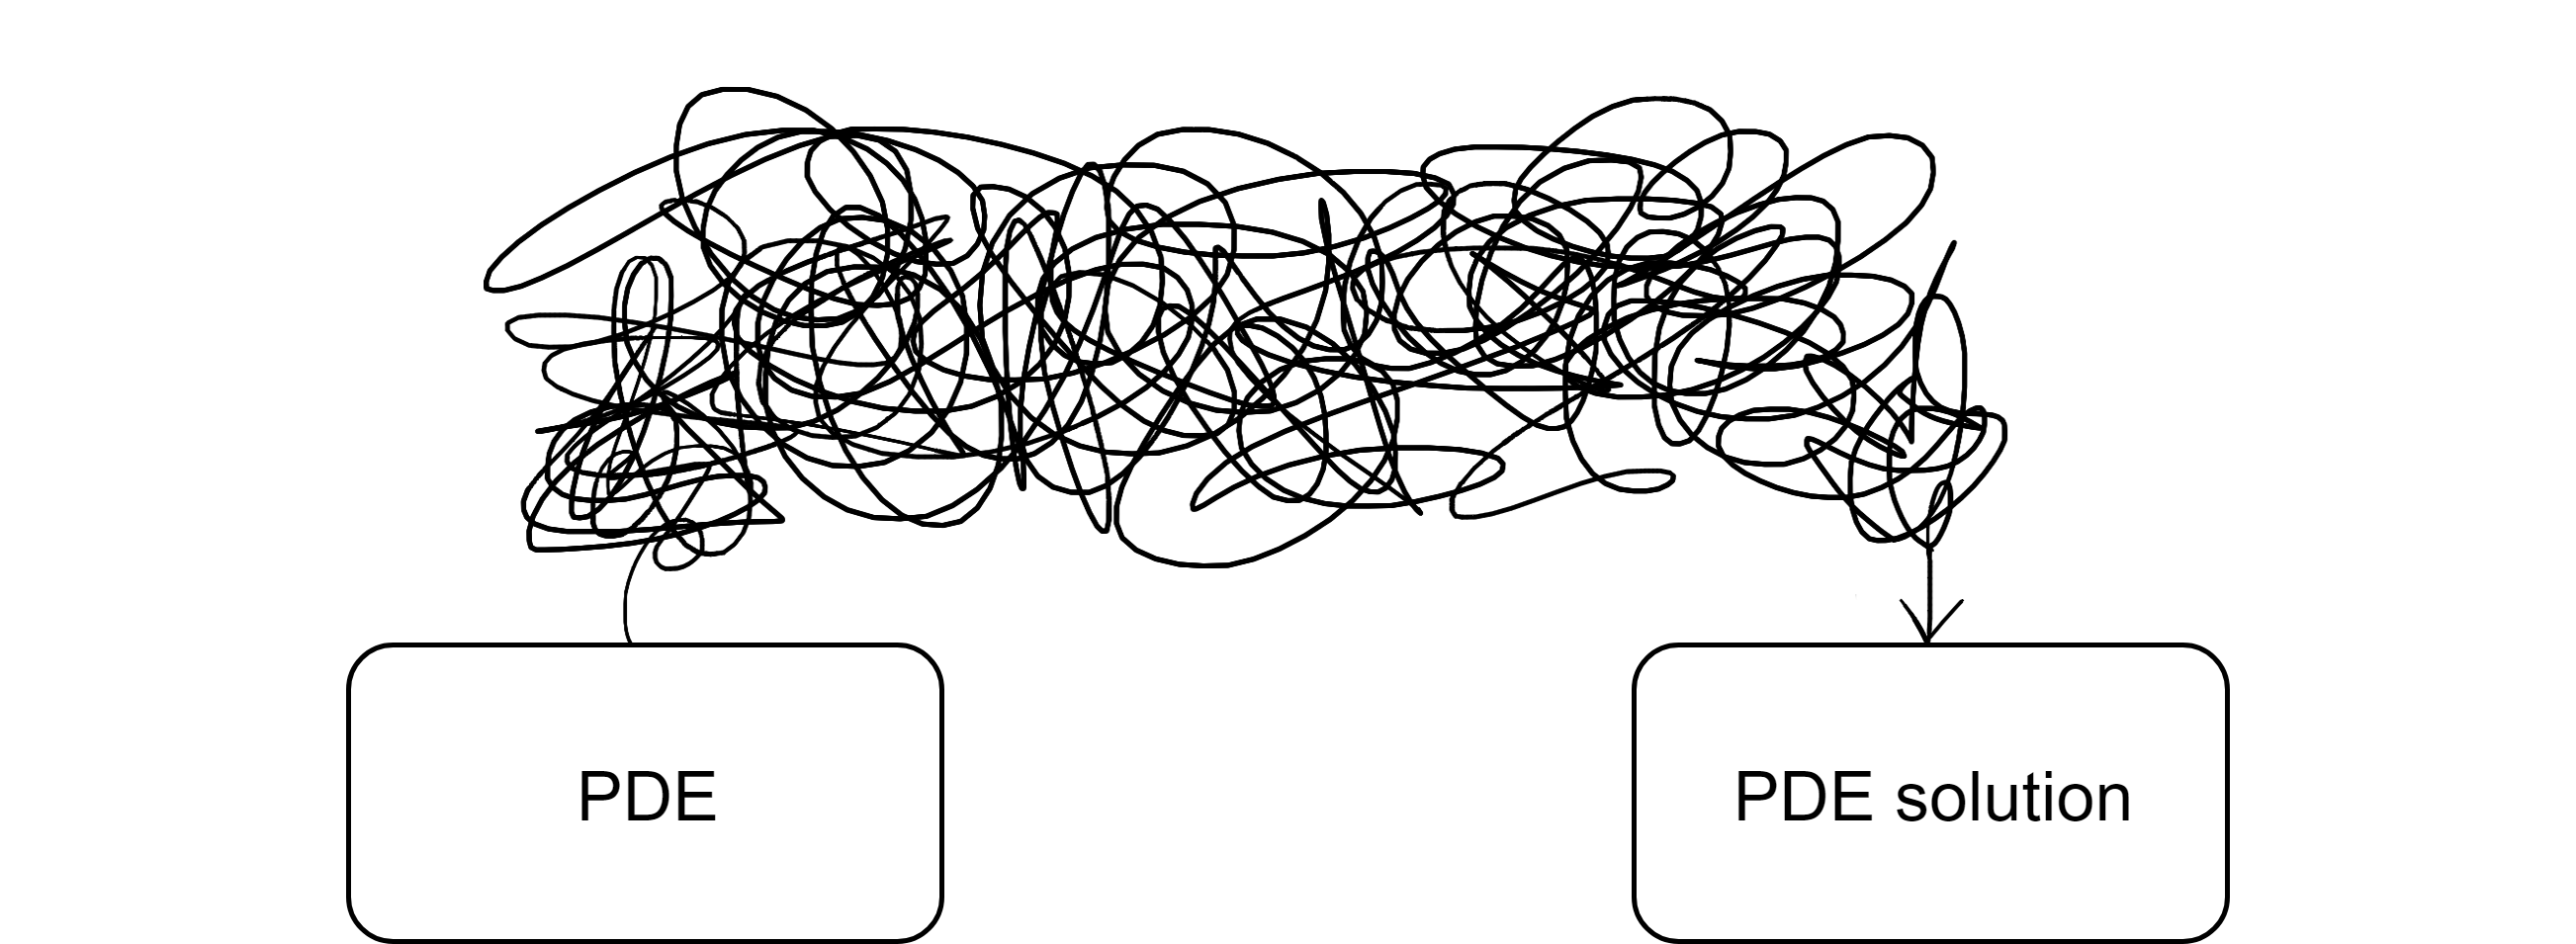
\includegraphics[width=1\textwidth]{transform_pairs_no_transform_pair.png}
    \end{figure}
\end{frame}

\begin{frame}
    \frametitle{Motivation}
    \begin{itemize}
        \item The Fokas method extends the idea of classical transform pair to a class of complicated IBVPs by constructing transform pairs depending on the problems' parameters.
        \begin{itemize}
            \item Even better, this class of IBVPs can have arbitrary spatial order.
        \end{itemize}
    \end{itemize}
    \begin{figure}[htpb!]
        \centering
        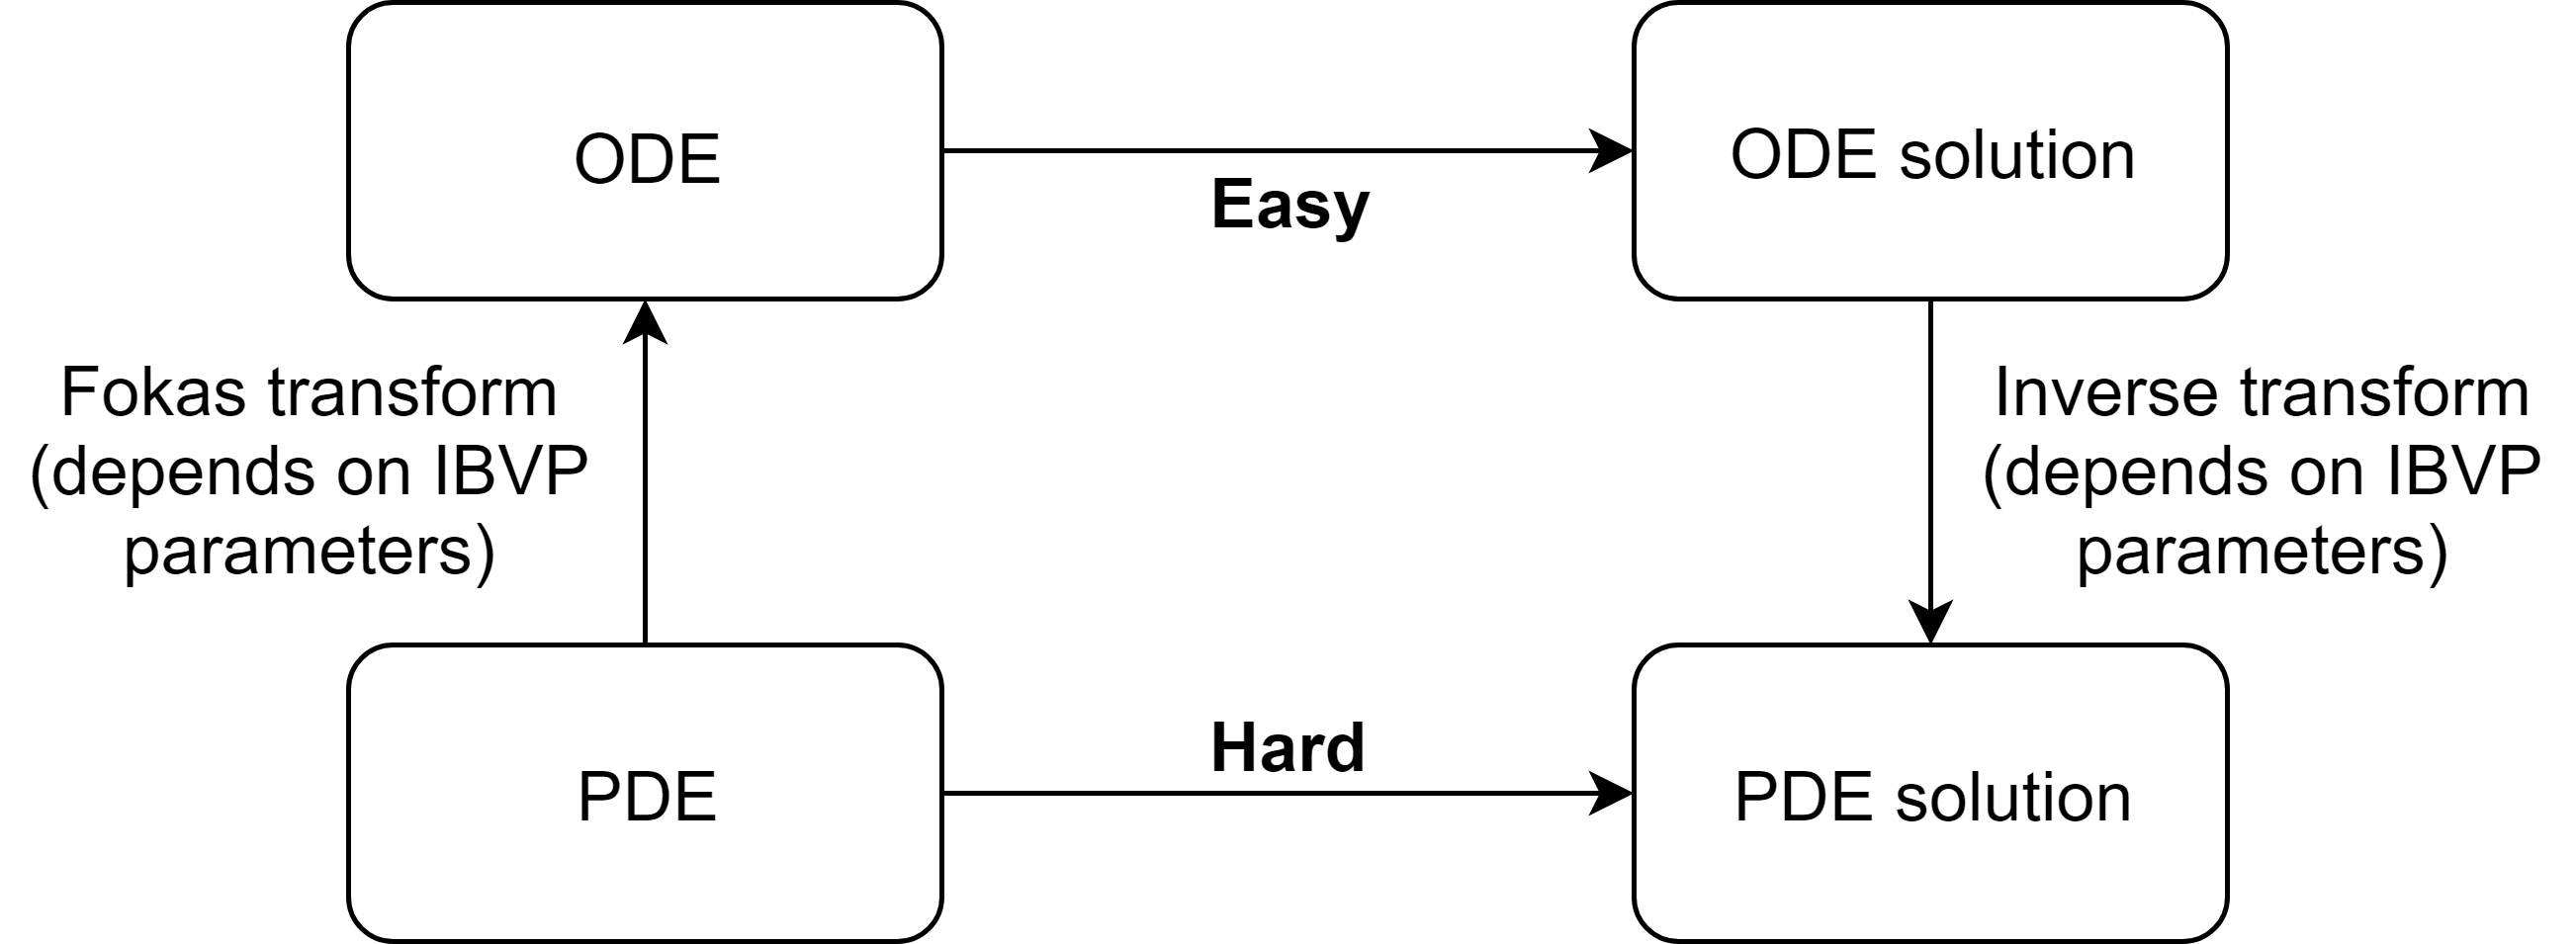
\includegraphics[width=1\textwidth]{fokas_transform.png}
        %\caption{Solving IBVPs using the Fokas transform pairs.}
        \label{fig:fokas_transform}
    \end{figure}
\end{frame}

\begin{frame}[t]
    \frametitle{Motivation}
    \begin{itemize}
        \item The Fokas method advances the understanding of high order PDEs by providing an algorithmic procedure to solve an entire class of IBVPs of arbitrary spatial order.
        \item However, it is still laborious to use the Fokas method by hand.
    \end{itemize}
    % Thus, capstone:
    % \begin{tcolorbox}[colback=white,colframe=gray!40, arc=0pt, outer arc=0pt]
    %     \begin{center}
    %         Implement the Fokas method as a software library$^*$ that supplies various computer aid in the process of solving IBVPs$^{**}$.
    %     \end{center}
    % \end{tcolorbox}
    % \begin{itemize}
    %     \item[$*$] In Julia: Being open-source allows for checking correctness.
    %     \item[$**$] This is the first time that the Fokas method is implemented computationally in any generality, and it allows solving a class of IBVPs for which no other solver algorithm yet exists.
    % \end{itemize}
\end{frame}

\begin{frame}[t]
    \frametitle{Motivation}
    \begin{itemize}
        \item The Fokas method advances the understanding of high order PDEs by providing an algorithmic procedure to solve an entire class of IBVPs of arbitrary spatial order.
        \item However, it is still laborious to use the Fokas method by hand.
    \end{itemize}
    \medskip
    Thus, capstone:
    \begin{tcolorbox}[colback=white,colframe=gray!40, arc=0pt, outer arc=0pt]
        \begin{center}
            Implement the Fokas method\textsuperscript{1} as a software library\textsuperscript{2} that supplies various computer aid\textsuperscript{3} in the process of solving IBVPs\textsuperscript{4}.
        \end{center}
    \end{tcolorbox}
    \begin{itemize}
        \item[] \textsuperscript{1}This is the first time that the Fokas method is implemented computationally in any generality.
        \item[] \textsuperscript{2}In Julia: Open-source allows for checking correctness.
        \item[] \textsuperscript{3}Numeric and symbolic features.
        \item[] \textsuperscript{4}For this class of IBVPs, no other solver algorithm yet exists.
    \end{itemize}
\end{frame}

\section{IBVPs solvable by the Fokas method}
\begin{frame}[t]
    \frametitle{IBVPs solvable by the Fokas method}
    %\small
    The Fokas method allows solving any well-posed IBVP of the form
    \begin{subequations}\label{eq:IBVP}
        \begin{alignat}{3}
            \left(\partial_t + a(-i)^n \partial_x^n\right)q(x,t) &= 0\quad &\forall (x,t)&\in (0,1)\times (0,T) \\
            q(x,0) &= f(x)\in \Phi\quad &\forall x&\in [0,1]\\
            q(\cdot, t) &\in \Phi \quad &\forall t&\in [0,T],
        \end{alignat}
    \end{subequations}
    where
    \begin{itemize}
        \item $a\in\C$ (for the IBVP to be well-posed, we require at least that $a=\pm i$ if $n$ is odd and $\real(a)\geq 0$ if $n$ is even),
        \item $\Phi$ is a set of functions that satisfy a set of homogeneous boundary conditions \begin{equation*}%\label{eq:Phi}
            \Phi:=\{\phi\in C^\infty[0,1]:\, B_j\phi = 0\,\forall j\in\{1,2,\ldots,n\}\},
        \end{equation*} 
        where $B_j$-s are boundary forms with boundary coefficients $b_{jk}$, $\beta_{jk}\in\R$,
        \begin{equation*}%\label{eq:B_j}
            B_j\phi := \sum_{k=0}^{n-1}\left(b_{jk}\phi^{(k)}(0) + \beta_{jk}\phi^{(k)}(1)\right),\, j\in\{1,2,\ldots,n\}.
        \end{equation*} 
    \end{itemize}
\end{frame}

% \begin{frame}[t]
%     \frametitle{IBVPs solvable by the Fokas method}
%     The Fokas method allows solving any well-posed IBVP that can be written in the form
%     %\begin{subequations*}\label{eq:IBVP}
%         \begin{alignat*}{3}
%             (\partial_t + a(-i)^n \frac{d^n}{dx^n})q(x,t) &= 0\quad &\forall (x,t)&\in (0,1)\times (0,T) \\
%             q(x,0) &= f(x)\in \Phi\quad &\forall x&\in [0,1]\\
%             q(\cdot, t) &\in \Phi \quad &\forall t&\in [0,T],
%         \end{alignat*}
%     %\end{subequations*}
%     where
%     \begin{itemize}
%         \item $\Phi$ is a space of functions that satisfy a set of homogeneous boundary conditions \begin{equation*}%\label{eq:Phi}
%             \Phi:=\{\phi\in C^\infty[0,1]:\, B_j\phi = 0\,\forall j\in\{1,2,\ldots,n\}\},
%         \end{equation*} 
%         where $B_j$-s are boundary forms
%         \begin{equation*}%\label{eq:B_j}
%             B_j\phi := \sum_{k=0}^{n-1}\left(b_{jk}\phi^{(k)}(0) + \beta_{jk}\phi^{(k)}(1)\right),\, j\in\{1,2,\ldots,n\},
%         \end{equation*}
%         and $b_{jk}$, $\beta_{jk}\in\R$. 
%     \end{itemize}
% \end{frame}

\begin{frame}[t]
    \frametitle{IBVPs solvable by the Fokas method}
    E.g., the linearized Korteweg-de Vries (KdV) equations:
    \newline

    \textbf{Problem 1}
    \begin{alignat*}{3}
        q_t(x,t) + q_{xxx}(x,t) &= 0,\quad &(x,t)&\in (0,1)\times (0,T)\\
        q(x,0) &= f(x),\quad &x&\in [0,1]\\
        q(0,t) = q(1,t) &= 0, \quad &t&\in [0,T]\\
        2q_x(1,t) &= q_x(0,t)\quad &t&\in [0,T].
    \end{alignat*}

    \textbf{Problem 2}
    \begin{alignat*}{3}
        q_t(x,t) + q_{xxx}(x,t) &= 0,\quad &(x,t)&\in (0,1)\times (0,T)\\
        q(x,0) &= f(x),\quad &x&\in [0,1]\\
        q(0,t) = q(1,t) = q_x(1,t) &= 0, \quad &t&\in [0,T].
    \end{alignat*}
\end{frame}

\section{Algorithm}
\begin{frame}[fragile]
    \frametitle{Algorithm: Overview}
    Consider an IBVP of the form
    %\begin{subequations*}\label{eq:IBVP}
        \begin{alignat*}{3}
            \left(\partial_t + a(-i)^n \partial_x^n \right)q(x,t) &= 0\quad &\forall (x,t)&\in (0,1)\times (0,T) \\
            q(x,0) &= f(x)\in \Phi\quad &\forall x&\in [0,1]\\
            q(\cdot, t) &\in \Phi \quad &\forall t&\in [0,T].
        \end{alignat*}
    %\end{subequations*}
    \begin{tcolorbox}[colback=white,colframe=gray!40, arc=0pt, outer arc=0pt]
        \begin{center}
            \begin{tikzpicture}
                \node[draw] at (0, 2.5) (ODE) [box] {$(\partial_t + a\lambda^n)\hat{q}(\lambda,t) = 0$\\ $\hat{q}(\lambda,0) = \hat{f}(\lambda)$};
                \node[draw] at (0, 0) (PDE) [box] {$(\partial_t + a(-i)^n \partial_x^n)q(x,t) = 0$\\$q(\cdot, t)\in\Phi$};
                \node[draw] at (6, 2.5) (ODE solution) [box] {$\hat{q}(\lambda,t)=e^{-a\lambda^n t}F_\lambda(f)$};
                \node[draw] at (6, 0) (PDE solution) [box] {$q(x,t) = f_x(e^{-a\lambda^n t}F_\lambda(f))$};
                \draw[arrow] (PDE) -- node[mylabel] {Transform $F_\lambda$} (ODE);
                \draw[arrow] (ODE) -- node[above] {Solve} (ODE solution);
                \draw[arrow] (ODE solution) -- node[mylabel] {Inverse transform $f_x$} (PDE solution);
                \draw[arrow,dashed] (PDE) -- (PDE solution);
            \end{tikzpicture}
        \end{center}
    \end{tcolorbox}
\end{frame}

\begin{frame}
    \frametitle{Algorithm: Overview}
    \begin{itemize}
        \item Input: An IBVP of the form
        %\begin{subequations*}\label{eq:IBVP}
            \begin{alignat*}{3}
                \left(\partial_t + a(-i)^n \partial_x^n \right)q(x,t) &= 0\quad &\forall (x,t)&\in (0,1)\times (0,T) \\
                q(x,0) &= f(x)\in \Phi\quad &\forall x&\in [0,1]\\
                q(\cdot, t) &\in \Phi \quad &\forall t&\in [0,T].
            \end{alignat*}
        %\end{subequations*}
        \item Construct adjoint boundary conditions of the spatial ordinary BVP.
        \item Using the spatial adjoint boundary conditions and other information about the IBVP, construct the Fokas transform pair $F_\lambda$ and $f_x$.
        \item Output: Solution of the IBVP $q(x,t) = f_x(e^{-a\lambda^n t}F_\lambda(f))$.
    \end{itemize}
\end{frame}

% \begin{frame}[t]
%     \frametitle{Algorithm: Constructing adjoint boundary conditions}
%     \textbf{Intuition}

%     Recall from linear algebra that, given a linear map $T$ from inner product spaces $V$ to $W$ (denoted as $T\in\mathcal{L}(V,W)$), the adjoint of $T$ is the function $T^\star:W\to V$ with
%         \begin{equation*}%\label{eq:linear map adjoint}
%             \langle Tv, w\rangle = \langle v, T^\star w\rangle
%         \end{equation*}
%         for $v\in V$, $w\in W$, where $\langle \cdot,\,\cdot \rangle$ denotes inner products defined on $V$ and $W$ \footcite[p.204]{Axler1997}.
% \end{frame}

% \begin{frame}[t]
%     \frametitle{Algorithm: Constructing adjoint boundary conditions}
%     \textbf{Intuition}
    
%     Similarly, given an ordinary differential equation BVP on $[a,b]$
%         \[Lx = 0,\quad Ux=0,\]
%         where $L$ is a linear differential operator of order $n$, the adjoint problem is 
%         \[L^+x = 0,\quad U^+x = 0,\]
%         where $L^+$ is the adjoint operator of $L$ and $U^+$ the adjoint boundary conditions of $U$, such that 
%         \[\langle Lu, v\rangle = \langle u, L^+v\rangle\]
%         for all $u, v\in C^n[a,b]$ such that $Uu=0$, $U^+v=0$.
% \end{frame}

\begin{frame}
    \frametitle{Algorithm: Constructing adjoint boundary conditions}
    %\textbf{Construction}

    An algorithm to find adjoint boundary conditions is developed based on literature\footcite{CoddingtonLevinson}, which includes (among definitions of various relevant objects)
    \begin{itemize}
        \item a constructive existence theorem on the adjoint, and
        \item a theorem to check whether a candidate adjoint is indeed valid.
    \end{itemize}
    These results are expanded and adapted to an algorithm to construct valid adjoint boundary conditions.
\end{frame}

\begin{frame}[t]
    \frametitle{Algorithm: Constructing Fokas transform pair}
    \textbf{Integrand construction}

    Let $b^\star, \beta^\star$ be the matrices associated with the adjoint boundary conditions.
    Let $\alpha := e^{2\pi i/n}$. For complex variable $\lambda$, define $n\times n$ matrices $W^+(\lambda)$, $W^-(\lambda)$ entry-wise by
    %\begin{subequations}\label{eq:M+/-}
        \begin{align*}
            W^+_{kj}(\lambda) &:= \sum_{r=0}^{n-1}(-i\alpha^{k-1}\lambda)^r b^\star_{jr}\\
            W^-_{kj}(\lambda) &:= \sum_{r=0}^{n-1}(-i\alpha^{k-1}\lambda)^r \beta^\star_{jr}.
        \end{align*}
    %\end{subequations}
    Define $n\times n$ matrix $W$ entry-wise by
    \begin{equation*}%\label{eq:M}
        W_{kj}(\lambda) := W^+_{kj}(\lambda) + W^-_{kj}(\lambda)e^{-\alpha^{k-1}\lambda}.
    \end{equation*}
    Define 
    \begin{equation*}%\label{eq:delta}
        \Delta(\lambda):=\det W(\lambda).
    \end{equation*}
\end{frame}

\begin{frame}[t]
    \frametitle{Algorithm: Constructing Fokas transform pair}
    \textbf{Integrand construction}
    
    Let $X^{lj}$ be the $(n-1)\times (n-1)$ submatrix of the block matrix $\mathbb{W}:=\begin{bmatrix}W & W\\ W & W\end{bmatrix}$, where $X^{lj}_{11}$ is $\mathbb{W}_{l+1, j+1}$.
    
    For $\lambda\in\C$ such that $\Delta(\lambda)\neq 0$, define the integrands
    %\begin{subequations}\label{eq:F_lambda_+-}
        \begin{align*}
            F^+_\lambda(f) &:= \frac{1}{2\pi \Delta(\lambda)} \sum_{j=1}^n\sum_{l=1}^n(-1)^{(n-1)(l+j)}\det X^{lj}(\lambda)W^+_{1j}(\lambda)\\
            &\qquad \int_0^1 e^{-i\alpha^{l-1}\lambda x}f(x)\,dx\\
            F^-_\lambda(f) &:= \frac{-e^{-i\lambda}}{2\pi \Delta(\lambda)} \sum_{j=1}^n\sum_{l=1}^n(-1)^{(n-1)(l+j)}\det X^{lj}(\lambda)W^-_{1j}(\lambda)\\
            &\qquad \int_0^1 e^{-i\alpha^{l-1}\lambda x}f(x)\,dx.
        \end{align*}
    %\end{subequations}
\end{frame}

\begin{frame}[t]
    \frametitle{Algorithm: Constructing Fokas transform pair}
    \textbf{Contour construction}
    
    Define the contours
        %\begin{subequations}\label{eq:gamma}
            \begin{align*}
                \Gamma_a^{\pm} &:= \partial(\{\lambda\in\C^{\pm}:\, \real(a\lambda^n)>0\}\setminus \bigcup_{\substack{\sigma\in\C;\\\Delta(\sigma)=0}} D(\sigma, 2\epsilon))\\
                \Gamma_a &:= \Gamma_a^+\cup \Gamma_a^-\\
                \Gamma_0^+ &:= \bigcup_{\substack{\sigma\in\cl\C^+;\\ \Delta(\sigma)=0}} C(\sigma, \epsilon)\\
                \Gamma_0^- &:= \bigcup_{\substack{\sigma\in\C^-;\\ \Delta(\sigma)=0}} C(\sigma, \epsilon)\\
                \Gamma_0 &:= \Gamma_0^+\cup \Gamma_0^-\\
                \Gamma &:= \Gamma_0\cup \Gamma_a.
            \end{align*}
        %\end{subequations}
\end{frame}

\begin{frame}[t]
    \frametitle{Algorithm: Constructing Fokas transform pair}
    \textbf{Contour construction}
    
    Sample contour drawn by hand\footcite{Smith2016}:
    \begin{figure}[htpb!]
        \centering
        \includegraphics[width=0.5\linewidth]{General-contours-02.mps}
        %\caption{Hypothetical $\Gamma$ contours corresponding to the case $a=-i$, taken from \cite{Smith2016}. The red dashed lines correspond to $\Gamma_a^+$, and the green dashed lines correspond to $\Gamma_a^-$. The blue circles correspond to $\Gamma_0^+$, and the black circles correspond to $\Gamma_0^-$. The arrows indicate the order of integration in equation \eqref{eq:q(x,t)_explicit}.}
        \label{fig:gamma_smith_fokas}
    \end{figure}
\end{frame}

\begin{frame}[t]
    \frametitle{Algorithm: Constructing Fokas transform pair}
    \textbf{Contour construction}

    Sample contours drawn by the implemented library\footcite{Xiao}:
    \begin{figure}
        \begin{subfigure}{.45\textwidth}
            \centering
            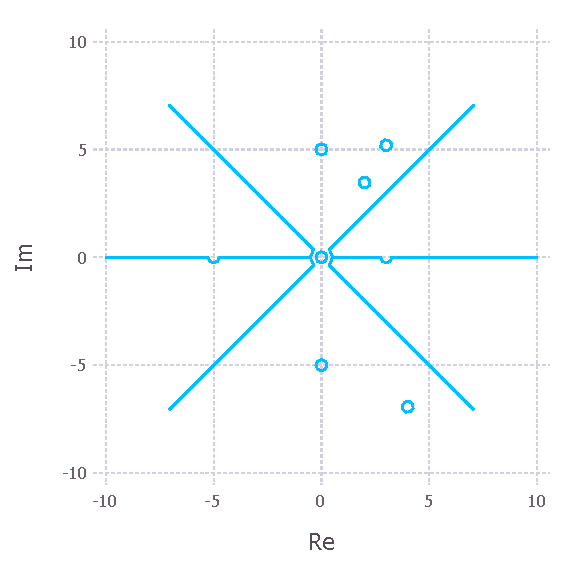
\includegraphics[width=1\linewidth]{contourPlot_n=2_a=1_cropped.pdf}
            \caption{$n=2$, $a=1$.}
        \end{subfigure}%
        \begin{subfigure}{.45\textwidth}
            \centering
            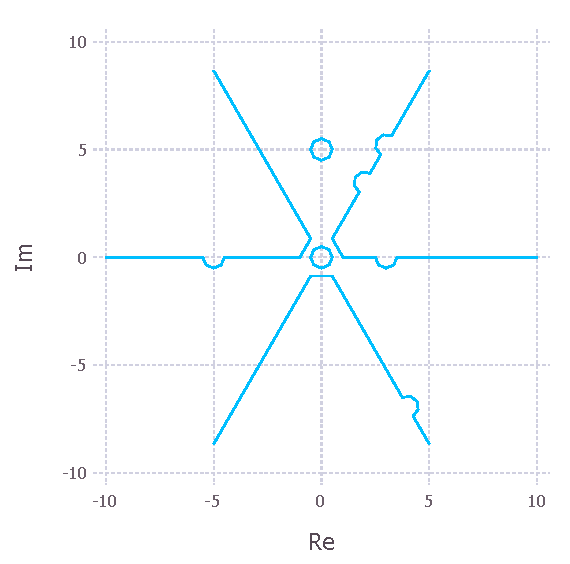
\includegraphics[width=1\linewidth]{contourPlot_n=3_a=-i_cropped.pdf}
            \caption{$n=3$, $a=-i$.}
        \end{subfigure}
        %\caption{$\Gamma$ with with zeroes of $\Delta(\lambda)$ at $3+3\sqrt{3}i$, $2+2\sqrt{3}i$, $0+0i$, $0+5i$, $0-5i$, $3$, $-5$, and $4-4\sqrt{3}i$. Note that $\Gamma_a^+$ are deformed to avoid zeroes on the sectors' boundaries.}
        %\label{fig:contourPlots}
    \end{figure}
\end{frame}

\begin{frame}[t]
    \frametitle{Algorithm: Constructing Fokas transform pair}
    \textbf{Contour construction}

    Sample contours drawn by the implemented library\footcite{Xiao}:
    \begin{figure}
        \begin{subfigure}{.45\textwidth}
            \centering
            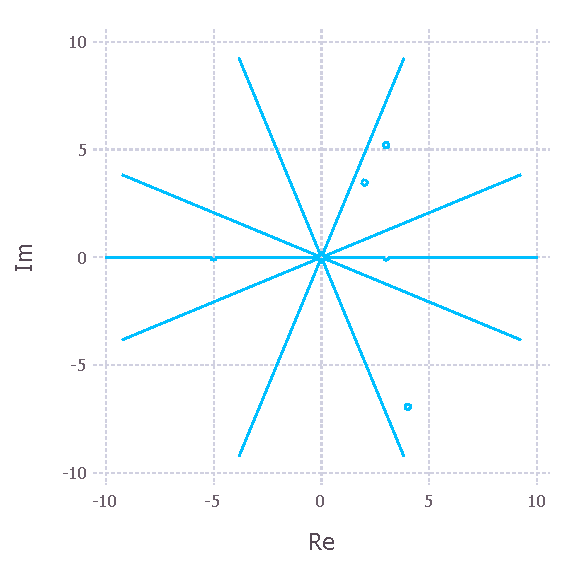
\includegraphics[width=1\linewidth]{contourPlot_n=4_a=1_cropped.pdf}
            \caption{$n=4$, $a=1$.}
        \end{subfigure}
        \begin{subfigure}{.45\textwidth}
            \centering
            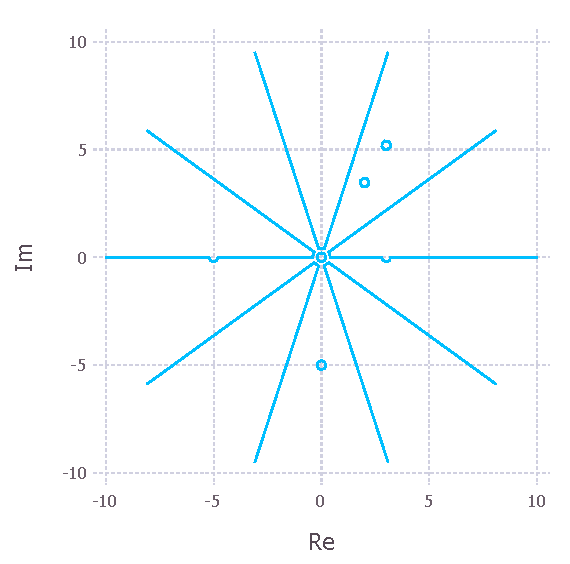
\includegraphics[width=1\linewidth]{contourPlot_n=5_a=-i_cropped.pdf}
            \caption{$n=5$, $a=-i$.}
        \end{subfigure}
    \end{figure}
\end{frame}

\begin{frame}
    \frametitle{Algorithm: Constructing Fokas transform pair}
    Define the Fokas transform pair
    %\begin{subequations}\label{eq:fokas_transform_pair}
        \begin{alignat*}{3}
            F_\lambda: f(x)&\mapsto F(\lambda)\quad &F_\lambda(f) &= \begin{cases}F^+_\lambda(f)\quad\mbox{if $\lambda\in \Gamma_0^+\cup \Gamma_a^+$},\\F^-_\lambda(f)\quad\mbox{if $\lambda\in \Gamma_0^-\cup \Gamma_a^-$},\end{cases}\\
            f_x:F(\lambda)&\mapsto f(x)\quad &f_x(F) &= \int_\Gamma e^{i\lambda x} F(\lambda)\,d\lambda,\, x\in [0,1].
        \end{alignat*}
    %\end{subequations}
\end{frame}

\begin{frame}
    \frametitle{Algorithm: IBVP solution}
    The solution to the IBVP is given by 
    \begin{equation*}
        \begin{split}
            q(x,t) &= f_x\left(e^{-a\lambda^n t}F_\lambda(f)\right)\\
            &= \int_{\Gamma_0^+}e^{i\lambda x}e^{-a\lambda^n t}F_\lambda^+(f)\,d\lambda + \int_{\Gamma_a^+}e^{i\lambda x}e^{-a\lambda^n t}F_\lambda^+(f)\,d\lambda\\
            &\qquad + \int_{\Gamma_0^-}e^{i\lambda x}e^{-a\lambda^n t}F_\lambda^-(f)\,d\lambda + \int_{\Gamma_a^-}e^{i\lambda x}e^{-a\lambda^n t}F_\lambda^-(f)\,d\lambda.
        \end{split}
    \end{equation*}
\end{frame}

\section{Sample usage}
\begin{frame}
    \frametitle{Sample usage: Solving IBVPs}
    \textbf{IBVP formulation}

    Consider the IBVP
    \begin{subequations}\label{eq:ex1}
        \begin{alignat}{3}
            q_t - q_{xx} &= 0\quad &\forall (x,t)&\in (0,1)\times (0,T) \label{eq:ex1_PDE}\\
            q(x,0) &= \sin(2\pi x) \quad &\forall x&\in [0,1]\label{eq:ex1_initial_condition}\\
            q(0,t) - q(1,t) &= 0 &\forall t&\in [0,T]\label{eq:ex1_boundary_condition1}\\
            q_x(0,t) - q_x(1,t) &= 0 &\forall t&\in [0,T]\label{eq:ex1_boundary_condition2}.
        \end{alignat}
    \end{subequations}
    Rewriting the IBVP in the standard form, we have $n=2$, $a=1$,
    \begin{align*}
    B_1\phi &= 1\cdot \varphi(0) + (-1)\cdot \varphi(1) + 0\cdot \varphi^{(1)}(0) + 0\cdot \varphi^{(1)}(1)\\
    B_2\phi &= 0\cdot \varphi(0) + 0\cdot \varphi(1) + 1\cdot \varphi^{(1)}(0) + (-1)\cdot \varphi^{(1)}(1),
    \end{align*}
    and
    \[\Phi = \{\phi\in C^{\infty}[0,1]:\, B_j\phi = 0\,\forall j\in\{1,2\}\}.\]
\end{frame}

\begin{frame}
    \frametitle{Sample usage: Solving IBVPs}
    \textbf{Adjoint boundary conditions construction}

    The matrices associated with the spatial adjoint boundary conditions are
    \[b^\star = \begin{bmatrix}0&-1\\ 1&0\end{bmatrix},\quad \beta^\star = \begin{bmatrix}0&1\\ -1&0\end{bmatrix}.\]

    \textbf{Fokas transform pair construction}

    We compute the integrands $F_\lambda^+(f)$, $F_\lambda^-(f)$ to be
    \[F_\lambda^+(f) = \frac{\left(\int_0^1 e^{i\lambda x}f(x)\,dx\right)e^{i\lambda}}{2\pi(e^{i\lambda}-1)},\quad F_\lambda^-(f) = \frac{\int_0^1 e^{i\lambda x}f(x)\,dx}{2\pi(e^{i\lambda}-1)}.\]
\end{frame}

\begin{frame}
    \frametitle{Sample usage: Solving IBVPs}
    \textbf{Fokas transform pair construction}

    We compute the contours to be:
    \begin{figure}[htpb!]
        \centering
        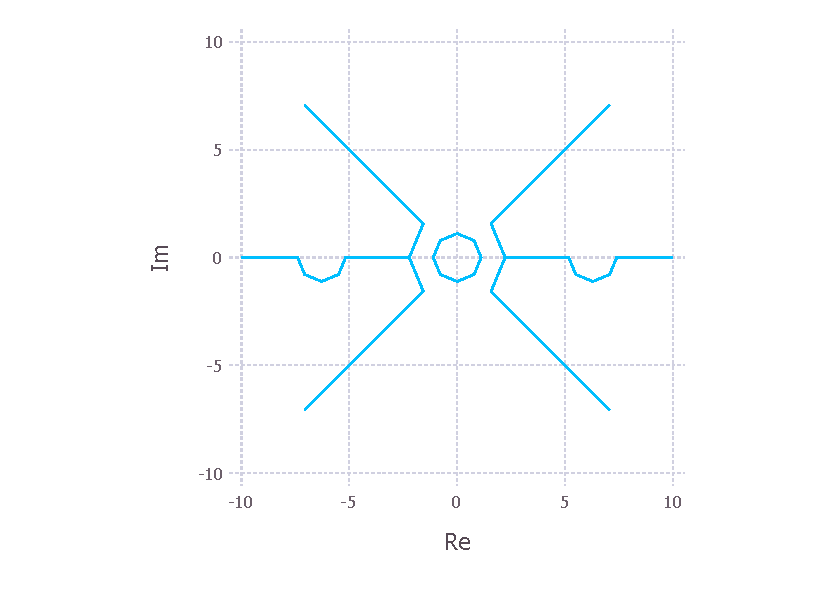
\includegraphics[width=0.7\linewidth]{ex1_contourPlot.pdf}
        % \caption{The $\Gamma$ contour.}
        % \label{fig:ex1_contourPlot}
    \end{figure}
    \textbf{IBVP solution}

    $q(x,t)$ can be evaluated within $20$s.
\end{frame}

\begin{frame}
    \frametitle{Sample usage: Symbolic features}
    Applying the Fokas method requires two technical lemmas concerning the poles of the integrands $F_\lambda^+$, $F_\lambda^-$ and their asymptotic behaviour \footcite{Miller2018}. 
    \newline

    Thus, it is necessary to obtain symbolic formulas for the integrands. 
    \newline

    In the case of complicated integrands, it is of interest to compute their symbolic formulas using a computer.
    \newline

    We verified that the library computes the correct symbolic formulas for $F_\lambda^+$, $F_\lambda^-$ using the following two problems.
\end{frame}

\begin{frame}
    \frametitle{Sample usage: Symbolic features}
    \textbf{Problem 1}
    \small
    \begin{alignat*}{3}
        q_t(x,t) + q_{xxx}(x,t) &= 0,\quad &(x,t)&\in (0,1)\times (0,T)\\
        q(x,0) &= f(x),\quad &x&\in [0,1]\\
        q(0,t) &= 0 = q(1,t), \quad &t&\in [0,T]\\
        2q_x(1,t) &= q_x(0,t)\quad &t&\in [0,T],
        \end{alignat*}
        with
        \begin{align*}
        F_\lambda^+(f) &= \frac{1}{2\pi\Delta(\lambda)}\left[\hat{f}(\lambda)(e^{i\lambda} + 2\alpha e^{-i\alpha\lambda} + 2\alpha^2 e^{-i\alpha^2\lambda}) + \hat{f}(\alpha\lambda)(\alpha e^{i\alpha\lambda} - 2\alpha e^{-i\lambda}) \right.\\
        &\qquad \left. + \hat{f}(\alpha^2\lambda)(\alpha^2e^{i\alpha\lambda} - 2\alpha^2e^{-i\lambda})\right]\\
        F_\lambda^-(f) &= \frac{e^{-i\lambda}}{2\pi\Delta(\lambda)}\left[-\hat{f}(\lambda)(2+\alpha^2 e^{-\alpha\lambda} + \alpha e^{-\alpha^2\lambda}) - \alpha\hat{f}(\alpha\lambda)(2-e^{-i\alpha^2\lambda}) \right.\\ 
        &\qquad \left. - \alpha^2\hat{f}(\alpha^2\lambda)(2-e^{-i\alpha\lambda})\right],
        \end{align*}
        where $\Delta(\lambda) = e^{i\lambda} + \alpha e^{i\alpha\lambda} + \alpha^2 e^{i\alpha^2\lambda} + 2(e^{-i\lambda} + \alpha e^{-i\alpha\lambda} + \alpha^2e^{-i\alpha^2\lambda})$ and $\hat{f}(\alpha^{l-1}\lambda) = \int_0^1 e^{-i\alpha^{l-1}\lambda x}f(x)\,dx$.
\end{frame}

\begin{frame}
    \frametitle{Sample usage: Symbolic features}
    \textbf{Problem 2}
    \small
    \begin{alignat*}{3}
        q_t(x,t) + q_{xxx}(x,t) &= 0,\quad &(x,t)&\in (0,1)\times (0,T)\\
        q(x,0) &= f(x),\quad &x&\in [0,1]\\
        q(0,t) &= 0, \quad &t&\in [0,T]\\
        q(1,t) &= 0\quad &t&\in [0,T]\\
        q_x(1,t) &= 0 \quad &t&\in [0,T],
        \end{alignat*}
        with
        \begin{align*}
        F_\lambda^+(f) &= \frac{1}{2\pi\Delta(\lambda)}\left[\hat{f}(\lambda)(\alpha e^{-\alpha\lambda} + \alpha^2 e^{-i\alpha^2\lambda}) - (\alpha\hat{f}(\alpha\lambda) + \alpha^2\hat{f}(\alpha^2\lambda))e^{-i\lambda}\right]\\
        F_\lambda^-(f) &= \frac{e^{-i\lambda}}{2\pi\Delta(\lambda)}\left[-\hat{f}(\lambda) - \alpha\hat{f}(\alpha\lambda) - \alpha^2\hat{f}(\alpha^2\lambda)\right],
        \end{align*}
        where $\Delta(\lambda) = e^{-i\lambda} + \alpha e^{-i\alpha\lambda} + \alpha^2e^{-i\alpha^2\lambda}$
        and $\hat{f}(\alpha^{l-1}\lambda) = \int_0^1 e^{-i\alpha^{l-1}\lambda x}f(x)\,dx$.
\end{frame}

\section{Discussion}
\begin{frame}
    \frametitle{Discussion}
    \begin{itemize}\setlength\itemsep{1em}
        \item Next step: Speed up
        \begin{itemize}
            \item Measures have been taken to bring down computation time to a reasonable range (e.g., by replacing double integral with explicit formulas).
            \item Yet to analyze the IBVP solution in-depth, evaluating it at a given $(x_0,t_0)$ should take less than milliseconds to allow graphing.
        \end{itemize}
        \item Idea: Develop a custom integrator tailored to the efficient evaluation of these contour integrals by exploiting the mathematical properties of the integrand and the contour.
    \end{itemize}
\end{frame}

\begin{frame}
    \frametitle{Summary}
    \begin{itemize}
        \item The Fokas method allows solving an entire class of IBVPs of arbitrary spatial order.
        \item A library has been developed in Julia to provide computer aid in the process of applying the Fokas method to solve IBVPs. These include symbolic formulas of important mathematical objects, their numeric approximations, and contour visualization. Code, unit tests, and documentations are available on a public GitLab repository\footcite{Xiao}.
        \item Looking ahead, it is of interest to develop a custom integrator to bring the computation time from dozens of seconds to the order of milliseconds.
    \end{itemize}
\end{frame}

% \begin{frame}{Bibliography}
% \bibliographystyle{utphys}
% \bibliography{C:/Bibtex/Capstone}
% \end{frame}

% \begin{frame}[t,allowframebreaks]
%     \frametitle{Bibliography}
%     \printbibliography
% \end{frame}

%----------------------------------------------------------------------------------------

\end{document} 